\documentclass{report}
\usepackage{graphicx}
\graphicspath{ {./images/} }
\usepackage[nottoc]{tocbibind}
\usepackage{blindtext}
\usepackage{booktabs}% http://ctan.org/pkg/booktabs
\newcommand{\tabitem}{~~\llap{\textbullet}~~}
\usepackage{geometry}
\geometry{
	a4paper,
	total={170mm,257mm},
	left=30mm,
	right=30mm,
	top=20mm,
}
\usepackage{array}

\begin{document}
	\begin{titlepage}
		\centering
		
\includegraphics[width=0.5\textwidth]{unipi.png}\par\vspace{1cm}
		{\scshape\LARGE Department of Information Engineering \par}
		\vspace{1cm}
		{\huge\bfseries Information Systems \par Task 0 Documentation  \par}
		\vspace{2cm}
		\vfill
		{\Large\scshape Students: \par 
			Adriano Botti \par
			Antonio Le Caldare \par
			Francesco Merola \par 
			Giacomo Ponziani \par}
		\vfill
		
	\end{titlepage}
\tableofcontents
\newpage
\listoffigures

\addcontentsline{toc}{chapter}{Application Specifications}
\chapter*{Application Specifications}
The goal of the application that we implemented is to provide a way for both students and professors to manage the registration process for exams. More specifically, we want the application to exert the following functionalities:
\begin{itemize}
	\item For Students:
	\begin{enumerate}
		\item Check past exams results
		\item Register to an exam date
		\item Delete an exam registration
	\end{enumerate}
	\item For Professors:
	\begin{enumerate}
		\item Add grades to an exam
		\item Create a new exam date
	\end{enumerate} 
\end{itemize}
The application is realized using the Java language, with the JavaFX extension to manage a graphic interface. The back-end uses a MySQL database to store the information.

\addcontentsline{toc}{chapter}{Requirements and Use Cases}
\chapter*{Requirements and Use Cases}
\addcontentsline{toc}{section}{Functional Requirements}
\section*{Functional Requirements}
The Professor:
\begin{enumerate}
	\item shall be able to insert an exam, associated with a course he holds, in a date of choice
	\item shall not be able to inster an exam for a date precedent to the current date
	\item shall be able to insert the corresponding grade for a student in his registration for that exam.
	\item shall insert all grades in the exact date of the exam
\end{enumerate}
The Student:
\begin{enumerate}
	\item shall be able to check the results of past exams
	\item shall be able to register to an exam not yet took
	\item shall not be able to register to an exam after the exam date.
	\item shall be able to register to more successive exams for the same course
	\item If the student registered to successive exams for the same course he just got a mark for, then those future registrations shall be deleted
	\item shall be able to deregister from an exam he was previously registered to
	\item shall not be able to deregister from an exam alredy took
	\item shall not be able to deregister from an exam after the exam date.
\end{enumerate}

\section*{Non-Functional Requirements}
For the application we identified Consistency and Availability as the two most important non-functional requirements.
Both the requirements can be satisfied by the use of a RDBMS, since for our application we don't manage high volumes of data. For this reason we employed a MySQL DBMS to implement our back-end
\newpage
\section*{Use Case Diagram}
From the funtional requirements, a Use Case Diagram is derived. For more detail and a step-by-step description of the different scenarios, see chapter \textit{User's Manual}.
\begin{figure}[ht]
	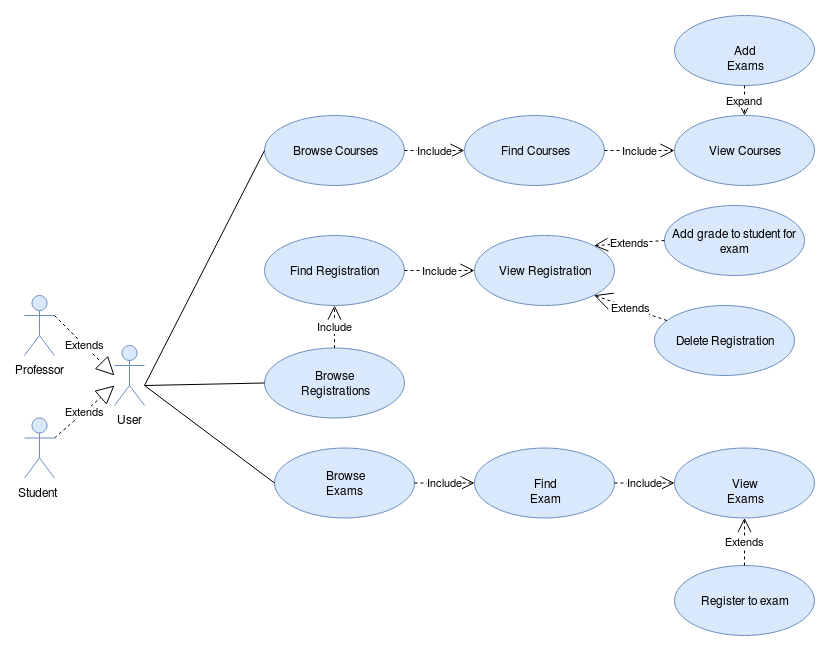
\includegraphics[width=1\textwidth]{UseCaseDiagram.png}
	\caption{Use Cases Diagram}
\end{figure}




\addcontentsline{toc}{chapter}{Entity-Relationship Diagram}
\chapter*{Entity-Relationship Diagram}
\addcontentsline{toc}{section}{ER Vocabulary}
\section*{ER Vocabulary}
\subsection*{Names definition}
Here we define in detail the terms for the main entites and relationships we will use in the following:
\begin{itemize}
	\item \textit{Student}\\ A student is an entity which is able to perform the operations already defined in the requirements. He's an actor for our application. 	
	\item \textit{Professor}\\ A professor is an entity which is able to perform the operations already defined in the requirements. He's an actor for our application. 	
	\item \textit{Course}\\ A course is held by one and only one professor. The course object only includes information about its name, cfu and the helding professor. It holds no information about when exams for that course will take place. 	
	\item \textit{Exam}\\ An exam represents the actual date of the examination for a course.
	\item \textit{Exam Result} An exam result relates an exam to all the students who registered to that exam, adding the information of the grade, if meaningful.\\
\end{itemize} 

\subsection*{Entities}
\begin{table}[ht]
	\centering
	\begin{tabular}{| m{6em} | m{15em} | m{8em} |}
		\hline
		\textbf{Entity} & \textbf{Description} & \textbf{Attributes} \\
		\hline
		Student & Holds all the information related to the students & 
		\tabitem $\underline{id}$ \\
		 & &\tabitem $name$ \\
		 & &\tabitem $surname$ \\
		\hline
		Professor & Holds all the information related to the professors & 
		\tabitem $\underline{id}$ \\
		& &\tabitem $name$ \\
		& &\tabitem $surname$ \\
		\hline
		Course & Holds the information related to the courses & 
		\tabitem $\underline{id}$ \\
		& &\tabitem $name$ \\
		& &\tabitem $cfu$ \\
		& &\tabitem $professor$ \\
		\hline
		Exam & Holds all the new and past exams& 
		\tabitem $\underline{course (ext)}$ \\
		& &\tabitem $\underline{date}$ \\
		\hline
	\end{tabular}
\end{table}

\newpage

\subsection*{Relationships}
\begin{table}[h]
	\centering
	\begin{tabular}{| m{6em} | m{14em} | m{8em} | m{7em} |}
		\hline
		\textbf{Relationship} & \textbf{Description} & \textbf{Participants} & \textbf{Attributes} \\
		\hline
		Teaching & Links Professors to their held courses & 
		\tabitem Professor(1,N) & \\ & &
		\tabitem Course(1,1) & \\
		\hline
		Exam Result & Links students to exams, with the respective grade & 
		\tabitem Student(0,N) & \tabitem $grade$ \\ & &
		\tabitem Exam(0,N) & \\
		\hline
		Exam Date Creation & Links the courses to the exams through a date & 
		\tabitem Course(0,N) & \\ & & 
		\tabitem Exam(1,1) & \\
		\hline
	\end{tabular}
\end{table}
\vspace{5em}
\addcontentsline{toc}{section}{ER Diagram}
\section*{ER Diagram}
\vspace{2em}
\begin{figure}[ht]
	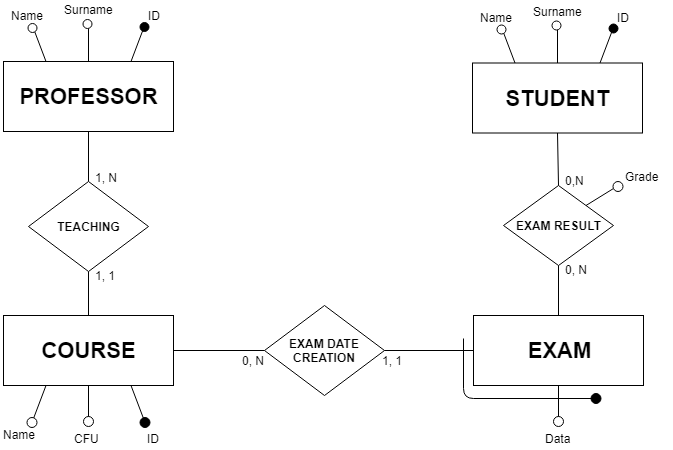
\includegraphics[width=1\textwidth]{ER_Diagram.png}
	\caption{Entity - Relationship Diagram}
\end{figure}

\addcontentsline{toc}{chapter}{UML Class Diagram}
\chapter*{UML Class Diagram} 
\begin{figure}[ht]
	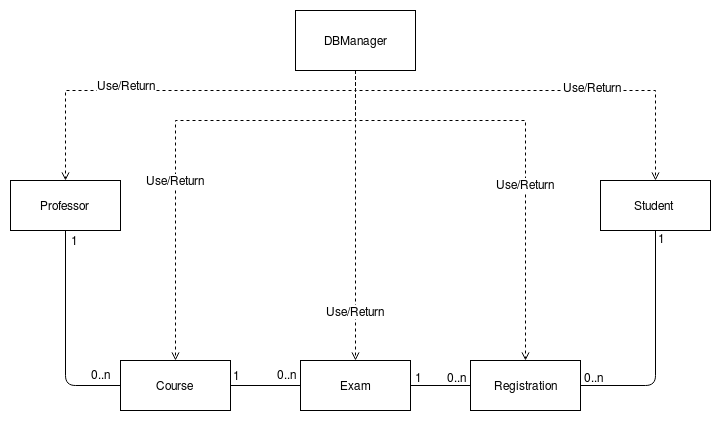
\includegraphics[width=1\textwidth]{ClassDiagram.png}
	\caption{Entity - Relationship Diagram}
\end{figure} 

\addcontentsline{toc}{chapter}{User's Manual}
\chapter*{User's Manual}

\begin{thebibliography}{9}
\end{thebibliography}

\end{document}
